%
% FH Technikum Wien
% !TEX encoding = UTF-8 Unicode
%
% Erstellung von Master- und Bachelorarbeiten an der FH Technikum Wien mit Hilfe von LaTeX und der Klasse TWBOOK
%
% Um ein eigenes Dokument zu erstellen, müssen Sie folgendes ergänzen:
% 1) Mit \documentclass[..] einstellen: Master- oder Bachelorarbeit, Studiengang und Sprache
% 2) Mit \newcommand{\FHTWCitationType}.. Zitierstandard festlegen (wird in der Regel vom Studiengang vorgegeben - bitte erfragen)
% 3) Deckblatt, Kurzfassung, etc. ausfüllen
% 4) und die Arbeit schreiben (die verwendeten Literaturquellen in Literatur.bib eintragen)
%
% Getestet mit TeXstudio mit Zeichenkodierung ISO-8859-1 (=ansinew/latin1) und MikTex unter Windows
% Zu beachten ist, dass die Kodierung der Datei mit der Kodierung des paketes inputenc zusammen passt!
% Die Kodierung der Datei twbook.cls MUSS ANSI betragen!
% Bei der Verwendung von UTF8 muss dnicht nur die Kodierung des Dokuments auf UTF8 gestellt sein, sondern auch die des BibTex-Files!
%
% Bugreports und Feedback bitte per E-Mail an latex@technikum-wien.at
%
% Versionen
% *) V0.7: 9.1.2015, RO: Modeline angepasst und verschoben
% *) V0.6: 10.10.2014, RO: Weitere Anpassung an die UK
% *) V0.5: 8.8.2014, WK: Literaturquellen überarbeitet und angepasst
% *) V0.4: 4.8.2014, WK: Initalversion in SVN eingespielt
%
\documentclass[MES,Master,ngerman]{twbook}%\documentclass[Bachelor,BMR,german]{twbook}
\usepackage[utf8]{inputenc}
\usepackage[T1]{fontenc}
\usepackage{subcaption} 

%
% Bitte in der folgenden Zeile den Zitierstandard festlegen
\newcommand{\FHTWCitationType}{IEEE} % IEEE oder HARVARD möglich - wenn Sie zwischen IEEE und HARVARD wechseln, bitte die temorären Dateien (aux, bbl, ...) löschen
%
\ifthenelse{\equal{\FHTWCitationType}{HARVARD}}{\usepackage{harvard}}{\usepackage{bibgerm}}

% Definition Code-Listings Formatierung:
\usepackage[final]{listings}
\lstset{captionpos=b, numberbychapter=false,caption=\lstname,frame=single, numbers=left, stepnumber=1, numbersep=2pt, xleftmargin=15pt, framexleftmargin=15pt, numberstyle=\tiny, tabsize=3, columns=fixed, basicstyle={\fontfamily{pcr}\selectfont\footnotesize}, keywordstyle=\bfseries, commentstyle={\color[gray]{0.33}\itshape}, stringstyle=\color[gray]{0.25}, breaklines, breakatwhitespace, breakautoindent}
\lstloadlanguages{[ANSI]C, C++, [gnu]make, gnuplot, Matlab}

%Formatieren des Quellcodeverzeichnisses
\makeatletter
% Setzen der Bezeichnungen für das Quellcodeverzeichnis/Abkürzungsverzeichnis in Abhängigkeit von der eingestellten Sprache
\providecommand\listacroname{}
\@ifclasswith{twbook}{english}
{%
    \renewcommand\lstlistingname{Code}
    \renewcommand\lstlistlistingname{List of Code}
    \renewcommand\listacroname{List of Abbreviations}
}{%
    \renewcommand\lstlistingname{Quellcode}
    \renewcommand\lstlistlistingname{Quellcodeverzeichnis}
    \renewcommand\listacroname{Abkürzungsverzeichnis}
}
% Wenn die Option listof=entryprefix gewählt wurde, Definition des Entyprefixes für das Quellcodeverzeichnis. Definition des Macros listoflolentryname analog zu listoflofentryname und listoflotentryname der KOMA-Klasse
\@ifclasswith{scrbook}{listof=entryprefix}
{%
    \newcommand\listoflolentryname\lstlistingname
}{%
}
\makeatother
\newcommand{\listofcode}{\phantomsection\lstlistoflistings}

% Die nachfolgenden Pakete stellen sonst nicht benötigte Features zur Verfügung
\usepackage{blindtext}

%
% Einträge für Deckblatt, Kurzfassung, etc.
%
\title{Der Objekt Orientierte Ansatz in der Entwicklung von Eingebetteten Systemen}
\author{Ney Fränz, BSc}
\studentnumber{1610297013}
%\author{Titel Vorname Name, Titel\and{}Titel Vorname Name, Titel}
%\studentnumber{XXXXXXXXXXXXXXX\and{}XXXXXXXXXXXXXXX}
\supervisor{FH-Prof. Dipl.-Ing. Dr. Martin Horauer}
%\supervisor[Begutachter]{Titel Vorname Name, Titel}
%\supervisor[Begutachterin]{Titel Vorname Name, Titel}
%\secondsupervisor{Titel Vorname Name, Titel}
%\secondsupervisor[Begutachter]{Titel Vorname Name, Titel}
%\secondsupervisor[Begutachterinnen]{Titel Vorname Name, Titel}
\place{Wien}
\kurzfassung{
In der Entwicklung von eingebetteten Systemen hat sich in den letzten Jahren einiges getan. Moderne Programmiersprachen wie C/C++ haben sich in der embedded Entwicklung etabliert und aufwendiges programmieren in Assembler sollte nur noch in wenigen Fällen von Nöten sein. Diese Arbeit beschäftigt sich hauptsächlich mit der Frage, ob der Einsatz einer objektorientierten Programmiersprache auf Plattformen mit nur wenigen kBytes an Flash Speicher sinnvoll ist und welchen Mehrwert diese für die Embedded Entwicklung haben könnte. \newline \newline Hierbei sollen vor allem die gängigsten Konzepte (Klassen, Templates, etc.) der objektorientierten Sprache analysiert werden, um Solide Richtwerte über Performance und Speicherverbrauch geben zu können. Dazu soll der kompilierte Code analysiert und diverse Benchmark Tests durchgeführt werden. Zusätzlich wird der Vergleich mit einer klassischen funktionalen Programmiersprache dargestellt. \newline \newline Als Referenz Programmiersprache wird C/C++ in Verbindung mit der ARM Cortex-M Architektur verwendet, da diese Kombination sehr interessant für stromsparende und kleinere IoT Projekte ist und sich wahrscheinlich in Zukunft durchsetzen wird. Am Anfang wird auch eine State-Of-the-art Analyse über die momentan verfügbaren ARM C++ Compiler durchgeführt um auflisten zu können welche Versionen und Erweiterungen von C++ unterstützt werden.

}
\schlagworte{Objektorientiertes Programmieren, C/C++, Embedded Software, ARM Cortex-M}
\outline{\blindtext}
\keywords{Keyword1, Keyword2, Keyword3, Keyword4}
\acknowledgements{\blindtext}

\begin{document}


%Festlegungen für den HARVARD-Zitierstandard
\ifthenelse{\equal{\FHTWCitationType}{HARVARD}}{
\bibliographystyle{Harvard_FHTW_MES}%Zitierstandard FH Technikum Wien, Studiengang Mechatronik/Robotik, Version 1.2e
\citationstyle{dcu}%Correct citation-style (Harvardand, ";" between citations, "," between author and year)
\citationmode{abbr}%use "et al." with first citation
\iflanguage{ngerman}{
    %Deutsch Neue Rechtschreibung
    \newcommand{\citepic}[1]{(Quelle: \protect\cite{#1})}%Zitat: Bild
    \newcommand{\citefig}[2]{(Quelle: \protect\cite{#1}, S. #2)}%Zitat: Bild aus Dokument
    \newcommand{\citefigm}[2]{(Quelle: modifiziert "ubernommen aus \protect\cite{#1}, S. #2)}%Zitat: modifiziertes Bild aus Dokument
    \newcommand{\citep}{\citeasnoun}%In-Line Zitiat entweder mit \citep{} oder \citeasnoun{}
    \newcommand{\acessedthrough}{Verf{\"u}gbar unter:}%Für URL-Angabe
    \newcommand{\acessedthroughp}{Verf{\"u}gbar bei:}%Für URL-Angabe (Geschützte Datenbank, Zugriff durch FH)
    \newcommand{\acessedat}{Zugang am}%Für URL-Datum-Angabe
    \newcommand{\singlepage}{S.}%Für Seitenangabe (einzelne Seite)
    \newcommand{\multiplepages}{S.}%Für Seitenangabe (mehrere Seiten)
    \newcommand{\chapternr}{K.}%Für Kapitelangabe
    \renewcommand{\harvardand}{\&}%Harvardand in Zitaten
    \newcommand{\abstractonly}{ausschließlich Abstract}
    \newcommand{\edition}{. Auflage}%Angabe der Auflage
}{
\iflanguage{german}{
    %Deutsch
    \newcommand{\citepic}[1]{(Quelle: \protect\cite{#1})}%Zitat: Bild
    \newcommand{\citefig}[2]{(Quelle: \protect\cite{#1}, S. #2)}%Zitat: Bild aus Dokument
    \newcommand{\citefigm}[2]{(Quelle: modifiziert "ubernommen aus \protect\cite{#1}, S. #2)}%Zitat: modifiziertes Bild aus Dokument
    \newcommand{\citep}{\citeasnoun}%In-Line Zitiat entweder mit \citep{} oder \citeasnoun{}
    \newcommand{\acessedthrough}{Verf{\"u}gbar unter:}%Für URL-Angabe
    \newcommand{\acessedthroughp}{Verf{\"u}gbar bei:}%Für URL-Angabe (Geschützte Datenbank, Zugriff durch FH)
    \newcommand{\acessedat}{Zugang am}%Für URL-Datum-Angabe
    \newcommand{\singlepage}{S.}%Für Seitenangabe (einzelne Seite)
    \newcommand{\multiplepages}{S.}%Für Seitenangabe (mehrere Seiten)
    \newcommand{\chapternr}{K.}%Für Kapitelangabe
    \renewcommand{\harvardand}{\&}%Harvardand in Zitaten
    \newcommand{\abstractonly}{ausschließlich Abstract}
    \newcommand{\edition}{. Auflage}%Angabe der Auflage
}{
    %Englisch
    \newcommand{\citepic}[1]{(Source: \protect\cite{#1})}%Zitat: Bild
    \newcommand{\citefig}[2]{(Source: \protect\cite{#1}, p. #2)}%Zitat: Bild aus Dokument
    \newcommand{\citefigm}[2]{(Source: taken with modification from \protect\cite{#1}, p. #2)}%Zitat: modifiziertes Bild aus Dokument
    \newcommand{\citep}{\citeasnoun}%In-Line Zitiat entweder mit \citep{} oder \citeasnoun{}
    \newcommand{\acessedthrough}{Available at:}%Für URL-Angabe
    \newcommand{\acessedthroughp}{Available through:}%Für URL-Angabe (Geschützte Datenbank, Zugriff durch FH)
    \newcommand{\acessedat}{Accessed}%Für URL-Datum-Angabe
    \newcommand{\singlepage}{p.}%Für Seitenangabe (einzelne Seite)
    \newcommand{\multiplepages}{pp.}%Für Seitenangabe (mehrere Seiten)
    \newcommand{\chapternr}{Ch.}%Für Kapitelangabe
    \renewcommand{\harvardand}{\&}%Harvardand in Zitaten
    \newcommand{\abstractonly}{Abstract only}
    \newcommand{\edition}{~edition}%Edition -> note, that you have to write "edition = {2nd},"!
}}}

\maketitle


%
% .. und hier beginnt die eigentliche Arbeit. Viel Erfolg beim Verfassen!
%
\chapter{State-of-Art Analyse}
Dieses Kapitel soll einen Überblick über aktuelle Mikrocontroller Architekturen und dessen Tools zur Entwicklung darstellen. Die Auswahl des richtigen Mikrocontrollers für ein Projekt ist eines der wichtigsten Schritte was einiges an Zeit und Recherche beansprucht. Auch das auswählen der richtigen Tooolchain oder die Frage ob ein RTOS oder OS zum Einsatz kommen soll wird immer wichtiger und hängt stark davon ab für welchen Mikrocontroller oder Architektur man sich entschieden hat. Stellt man während der Projektphase fest das der verwendete Mikrocontroller ungeeignet ist oder bestimmte Hardware Features fehlen, ist das meist ein großes Risiko welches den Erfolg des Projektes beeinflussen kann.  
\section{Mikrocontroller Hardware Analyse}
Dieses Kapitel soll die Hardware Features und die gängigsten CPU Architekturen näher beschreiben. Der Trend neigt dazu dass immer mehr Funktionalität welche früher als externe Peripherie an den Mikrocontroller angeschlossen werden musste in diesen integriert wird. Dies führt dazu dass moderne Mikrocontroller immer komplexer werden was die Verwendung von Softwarebibliotheken welche die Hardware ansprechen immer notwendiger macht. Auch Codegeneratoren mit denen man die komplexe Hardware über eine User Interface komfortabel konfigurieren kann finden immer mehr Einzug in die Entwicklungsumgebungen der verschiedenen Halbleiter Hersteller. Dieses Phänomen kann man gut an der Seitenanzahl vom Datenblatt gängiger Mikrocontroller erkennen. Hatten frühere 8 Bit Mikrocontroller noch 500 oder weniger Seiten findet man heute kaum noch ein Datenblatt mit weniger als 2000 Seiten. Auch die Energieeffizienz scheint eine immer wichtigere Rolle zu spielen was durch den steigernden Anteil von mobilen Geräten zu erklären ist. 
\subsection{8bit vs 32bit CPU}
\subsection{Stromverbrauch und Effizienz}
\subsection{MCU Peripherie}
\subsection{Sicherheits- Features}
\section{Work-Flow und Tools in der embedded Entwicklung}
\subsection{Entwicklungs- Umgebungen}
\subsection{Test und Qualitäts- Management}
\subsection{Code Generatoren}
\subsection{Low-Level Hardware Bibliotheken}
\section{Programmiersprachen für die embedded Entwicklung}
\subsection{Kompilierte Programmiersprachen}
\subsection{Interpretierte Programmiersprachen}
\section{Verfügbare C/C++ Compiler für die ARM Architektur}
\subsection{GNU Arm Embedded Toolchain}
\subsection{IAR Embedded Workbench}
\subsection{ARM Compiler}


\chapter{Embedded C++}
\section{Überblick}
In diesem Kapitel werden verschiedene Konzepte von C++ näher analysiert um klare Aussagen über Speicherverbrauch und Performance liefern zu können. Es soll zugleich als eine Art Guideline für Embedded Programmierer dienen um C++ effizient einsetzen zu können. \newline 

Die GNU ARM Embbedded Toolchain wird für diese Tests verwendet da Sie neben Compiler, Linker und Co. auch noch viele nützliche Tools zur Analyse mitliefert. Verschieden Tools die in den nachfolgenden Kapiteln zum Einsatz kommen werden in Tabelle \ref{tbl:analystools} aufgelistet.

\begin{table}[!htb]
	\centering
	\begin{tabular}{| l | c | r |}
		\hline
		\textbf{Tool}  & \textbf{Beschreibung} \\ \hline
		arm-none-eabi-g++           & C++ Compiler (Präprozessor , Kompiler, Linker) \\ \hline
		arm-none-eabi-gcc       	& C	  Compiler (Präprozessor , Kompiler, Linker) \\ \hline
		arm-mone-eabi-nm        	& Listet Symbole aus Objekt Dateien \\ \hline
		arm-none-eabi-objdump		& Zur erweiterten Analyse von Objekt Dateien \\ \hline
		arm-none-eabi-size			& Zeigt Größe der verschieden Link Segmente (Text, Data, BSS) \\ \hline
	\end{tabular}
	
	\caption{Analyse Tools}
	\label{tbl:analystools}
	% Verweis im Text mittels \ref{tbl:beispieltabelle}
	
\end{table}


\newpage
\section{Funktionen Überladen}
In C++ ist es erlaubt mehrere Funktionen mit dem gleichen Namen zu deklarieren, diese sich jedoch in ihrer Signatur unterscheiden müssen. Somit kann man bestehende Funktionen überladen, indem man die Datentypen oder Anzahl der Parameter verändert. Der Compiler sucht sich dann die Funktion mit der passenden Signatur heraus. 
\subsection{Beispiel} \label{beispiel:1}
Im folgendem Beispiel braucht man eine Funktion die jeweils 2 \textit{int} und \textit{double} Werte addieren kann. Im klassischen C müsste man jeweils 2 Funktionen deklarieren die sich in ihrem Namen unterscheiden, wohingegen man in C++ den gleichen Funktionsnamen erneut verwenden darf.
\begin{figure}[!htb]
	\begin{subfigure}[b]{0.5\textwidth}
		\lstset{language=C++,caption={C++ Beispiel}}
		\lstinputlisting{../Code_Samples/Funkionen_Uberladen/C++/main.cpp}
		\label{fig:1}
	\end{subfigure}
	%
	\begin{subfigure}[b]{0.5\textwidth}
		\lstset{language=C,caption={C Beispiel}}
		\lstinputlisting{../Code_Samples/Funkionen_Uberladen/C/main.c}
		\label{fig:2}
	\end{subfigure}
\end{figure}

\subsection{Analyse}
Beide Compiler generieren jeweils eine Funktion für \textit{int} (48 byte) und eine für \textit{double} (76 byte). Beim C++ Compiler kann man erkennen das dieser automatisch 2 verschiedene Funktionen mit dem Index 'ii' und 'dd' erstellt. Somit erzeugen Funktionsüberladungen keinen zusätzlichen Speicher Overhead. Auch lange Funktionsnamen können vermieden werden und die Wahrscheinlichkeit das man irrtümlicherweise die falsche Funktion verwendet sinkt erheblich.
\begin{figure}[!htb]
	\begin{subfigure}[b]{0.5\textwidth}
		\begin{lstlisting}[gobble=6, title={Analyse C++}, language=bash, numbers=none]
		$ arm-none-eabi-g++ -c -O0 main.cpp
		$ arm-none-eabi-nm main.o --print-size
		...
		00000030 0000004c t _ZL3adddd
		00000000 00000030 t _ZL3addii
		...
		\end{lstlisting}
	\end{subfigure}
	%
	\begin{subfigure}[b]{0.5\textwidth}
		\begin{lstlisting}[gobble=6, title={Analyse C}, language=bash, numbers=none]
		$ arm-none-eabi-gcc -c -O0 main.c
		$ arm-none-eabi-nm main.o --print-size
		...
		00000030 0000004c t add_d
		00000000 00000030 t add_i
		...
		\end{lstlisting}
	\end{subfigure}
\end{figure}

\subsection{Fazit}
Funktionsüberladungen erzeugen keinen Speicher Overhead und sind zu empfehlen wenn sich der Funktionsblock erheblich in verschiedenen Implementierungen unterscheidet. Ändern sich nur die Datentypen wie es in diesem Beispiel der Fall ist sind \textit{Funktionstemplates} zu bevorzugen. Ändert sich nur die Anzahl der Parameter kann man oftmals mit \textit{Standardparametern} (Default Arguments) wie es sie in C++ gibt eleganteren Code erzeugen.

\newpage
\section{Standardparameter}
Bei der Initialisierung von Hardware Modulen sind oft Standardparameter sinnvoll. Bei einer Seriellen Schnittelle ist die Konfiguration \textit{9600 8N1} für viele Anwendungen schon ausreichend. In C++ kann man Funktionsparameter mit festen Standardwerten versehen welche geltend sind sollte beim Funktionsaufruf das jeweilige Argument fehlen. Im klassischen C gibt es mehrere Möglichkeiten so ein Verhalten nach zu implementieren, jedoch ist dies ohne zusätzlichen Quellcode meist nicht möglich.

\subsection{Beispiel}          
Das folgende Beispiel zeigt wie man die Initialisierungsfunktion einer Seriellen Schnittstelle mit Standardwerten versehen kann. Sofort erkennbar ist das die gleiche Implementierung in C wesentlich unübersichtlicher wirkt. In der main Funktion werden die verschieden Möglichkeiten dargestellt wie man die Funktion aufrufen könnte.
\begin{figure}[!htb]
	\begin{subfigure}[b]{0.5\textwidth}
		\lstset{language=C++,caption={C++ Beispiel}}
		\lstinputlisting{../Code_Samples/Standardparameter/C++/main.cpp}
		\label{fig:3}
	\end{subfigure}
	%
	\begin{subfigure}[b]{0.5\textwidth}
		\lstset{language=C,caption={C Beispiel}}
		\lstinputlisting{../Code_Samples/Standardparameter/C/main.c}
		\label{fig:4}
	\end{subfigure}
\end{figure}

\subsection{Analyse}
Bei dieser Analyse ist die Größe der \textit{main} Funktion im ROM wichtig, da in dieser die \textit{uart\_init} Funktion aufgerufen wird. Der C und C++ Compiler allozieren jeweils 240 Byte für die \textit{main} Funktion in der \textit{.text} Sektion. Analysiert man den generierten Assembler Code der \textit{main} Funktion von beiden Compilern kann man keinen Unterschied feststellen. Somit ergänzt der C++ Compiler lediglich die nicht gegeben Argumente mit den Standard Parametern während des Kompilierens. Die \textit{uart\_init} Funktion alloziert in der C Version mehr Speicher da hier gegebenenfalls die Standardparameter noch gesetzt werden müssen.

\begin{figure}[!htb]
	\begin{subfigure}[b]{0.5\textwidth}
		\begin{lstlisting}[gobble=6, title={Analyse C++}, language=bash, numbers=none]
		$ arm-none-eabi-g++ -c -O0 main.cpp
		$ arm-none-eabi-nm a.out --print-size
		...
		00000000 00000048 t _ZL9uart_initiiii
		00000000 000000f0 T main
		00000000 00000004 B ret
		...
		\end{lstlisting}
	\end{subfigure}
	%
	\begin{subfigure}[b]{0.5\textwidth}
		\begin{lstlisting}[gobble=6, title={Analyse C}, language=bash, numbers=none]
		$ arm-none-eabi-gcc -c -O0 main.c
		$ arm-none-eabi-nm a.out --print-size
		...
		00000000 00000098 t uart_init
		00000000 000000f0 T main
		00000000 00000004 B ret
		...
		\end{lstlisting}
	\end{subfigure}
\end{figure}
Bei Verwendung von C++ Standardparametern sollte man darauf achten dass man die Parameter, wo die Wahrscheinlichkeit einer Änderung am Höchsten ist möglichst links in die Funktionsparameter-Liste packt. Bei der Seriellen Schnittelle wäre das die Baudrate da sich die restlichen Parameter nicht so häufig ändern.  

\subsection{Fazit}
Standardparameter sind sehr nützlich wenn es sich um Konfigurations-Funktionen handelt da man diese übersichtlicher gestalten kann. Auch Funktions- Aufrufe mit langen Parameter Listen kann man vermeiden wenn einem die Standard Werte genügen. Einen Speicher Overhead oder Änderungen in der Laufzeit des Programms sind nicht zu befürchten.

\newpage

\section{Funktions- Templates}
Oftmals muss man eine und dieselbe Funktion für verschiedene Datentypen implementieren. In C++ kann man dieses Problem mit Templates sehr elegant lösen. Templates stellen eine Art Schablone dar mit denen man Funktionen unabhängig von einem bestimmten Datentypen implementieren kann. Dies ist vor allem bei Manipulationen von Listen oder Arrays interessant da man den Algorithmus nicht für jeden Datentypen erneut implementieren muss.

\subsection{Beispiel}
Das nachfolgende Beispiel zeigt wie man in C++ eine Funktion die 2 Werte addieren soll unabhängig von dessen Datentypen implementieren kann. Erkennbar ist auch dass die C++ Variante wesentlich kürzer und somit auch übersichtlicher als die Version in C wirkt.
\begin{figure}[!htb]
	\begin{subfigure}[b]{0.5\textwidth}
		\lstset{language=C++,caption={C++ Beispiel}}
		\lstinputlisting{../Code_Samples/Funkions_Templates/C++/main.cpp}
		\label{fig:5}
	\end{subfigure}
	%
	\begin{subfigure}[b]{0.5\textwidth}
		\lstset{language=C,caption={C Beispiel}}
		\lstinputlisting{../Code_Samples/Funkions_Templates/C/main.c}
		\label{fig:6}
	\end{subfigure}
\end{figure}
\subsection{Analyse}

Beide Versionen wurden mit der Compiler Optimierung \textit{-O0} kompiliert. Analysiert man beide Objekt Dateien findet man jeweils 2 Versionen von der Addier-Funktion. Bei der C Variante heißen die Funktionen genau gleich wie im Quellcode deklariert, wohingegen eine automatische Indexierung bei der C++ Variante erfolgt. In beiden Versionen werden jeweils 48 Byte für die \textit{int} und 76 Byte für die \textit{double} Funktion alloziert. Es kann durchaus sein dass bei anderen Optimierungsstufen die Funktionen als \textit{inline} kompiliert werden, jedoch entsteht auch dann nie ein Unterschied zwischen der C und C++ Version.


\begin{figure}[!htb]
	\begin{subfigure}[b]{0.5\textwidth}
		\begin{lstlisting}[gobble=6, title={Analyse C++}, language=bash, numbers=none]
		$ arm-none-eabi-g++ -c -O0 main.cpp
		$ arm-none-eabi-nm a.out --print-size
		...
		00000000 0000004c W _Z3addIdET_S0_S0_
		00000000 00000030 W _Z3addIiET_S0_S0_
		...
		\end{lstlisting}
	\end{subfigure}
	%
	\begin{subfigure}[b]{0.5\textwidth}
		\begin{lstlisting}[gobble=6, title={Analyse C}, language=bash, numbers=none]
		$ arm-none-eabi-gcc -c -O0 main.c
		$ arm-none-eabi-nm a.out --print-size
		...
		00000030 0000004c T add_d
		00000000 00000030 T add_i
		...
		\end{lstlisting}
	\end{subfigure}
\end{figure}

Zudem kann man erkennen das die Funktionen in der C Version mit \textit{t} markiert sind und somit in die \textit{.text} Sektion gelinkt werden. Würde man in einer anderen C Datei genau die gleiche Funktionen implementieren würde man nach dem linken 2 Versionen von genau der gleichen Funktion in der auszuführenden Datei (Executable) finden. Hierbei sind die Funktionen a und b fest an die jeweilige Objektdatei gebunden. In der C++ Version sind beide Funktionen als \textit{WEAK} deklariert und befinden sich in einer eigenen Link Sektion. Dies ermöglicht es dem Linker Optimierungen vorzunehmen falls es mehrere Implementierungen des gleichen Templates in verschieden Objekt Dateien gibt. Dieses Compiler Verhalten ist auch unter dem Namen \textbf{Borland Model} bekannt.

\begin{figure}[!htb]
	\begin{subfigure}[b]{0.5\textwidth}
		\begin{lstlisting}[gobble=6, title={Analyse C++}, language=bash, numbers=none]
		$ arm-none-eabi-objdump -d main.o

		-> .text:
		00000000 <main>:
		...
		-> .text._Z3addIhET_S0_S0_:
		00000000 <_Z3addIhET_S0_S0_>:
		...
		-> .text._Z3addIsET_S0_S0_:
		00000000 <_Z3addIsET_S0_S0_>:
		...
		
		\end{lstlisting}
	\end{subfigure}
	%
	\begin{subfigure}[b]{0.5\textwidth}
		\begin{lstlisting}[gobble=6, title={Analyse C}, language=bash, numbers=none]
		$ arm-none-eabi-objdump -d main.o
		
		-> .text:
		00000088 <main>:
		...
		
		00000000 <a>:
		...
		
		00000040 <b>:
		...
		\end{lstlisting}
	\end{subfigure}
\end{figure}

\subsection{Fazit}
Funktionstemplates erhöhen die Lesbarkeit des Quellcodes und bewirken das man Fehler nur in einer Funktion beheben muss was die Wartbarkeit erheblich erhöht. Zudem kann sich die Verwendung von Templates positiv auf die Größe des Executables auswirken da der Linker Optimierungen vornehmen kann. Templates sollten auch wenn möglich in einer header Datei definiert werden und wenn nötig in der .cpp Datei eingebunden werden. Bei großen Projekten kann sich dies jedoch negativ auf die Übersetzungszeit auswirken da der Template Code mehrmals kompiliert werden muss.
\newpage

\section{Die Standardbibliothek}
Dieses Kapitel widmet sich der Standardbibliothek welche ein wichtiger Bestandteil von C++ darstellt. Einige Begriffe welche im Zusammenhang mit der Bibliothek öfters genannt werden sollen hier näher beschrieben werden und auch die Frage ob sich der Einsatz in embedded Projekten lohnt soll hier beantwortet werden.
\subsection{Überblick}
Die Standardbibliothek is ein fester Bestandteil von C++ und wird von der ISO Organisation verwaltet. Diese wurde ursprünglich unter dem Namen STL (Standard Template Library) von Hewlett-Packard entwickelt und in den C++ Standard integriert. Jedoch handelt es sich nach wie vor um 2 getrennte Bibliotheken die parallel weiterentwickelt werden. Die C++ Standardbibliothek beinhaltet nützliche Funktionen und Algorithmen welche sehr beliebt sind. Zusätzlich beinhaltet die Standardbibliothek auch die komplette C Bibliothek. 

\subsubsection{Container-Klassen}
Container-Klassen sind generische Klassen welche andere Objekte und Datentypen speichern und verwalten können. Diese sind meistens als Template-Klassen implementiert wodurch man diese für die meisten Datentypen benutzen kann. Die bekanntestes Container sind \textit{std::vector} und \textit{std:array} welche auch in den nachfolgenden Kapiteln analysiert werden.
\subsubsection{Iteratoren}
An sich sind Iteratoren nichts anderes als intelligente Zeiger welche benutzt werden um durch die Elemente eines Container zu iterieren. Iteratoren sind reine Zugriffsobjekte und stellen die Schnittstelle für Algorithmen in C++ dar.
\subsubsection{Algorithmen}
Mit Algorithmen kann man Manipulationen an Container vornehmen. Diese sind Container unabhängig implementiert und benutzen Iteratoren um auf die Container Elemente zuzugreifen. Der \textit{std::for\_each} Algorithmus ist einer der bekanntesten mit dem man auf alle Elemente eines Containers Zugriff bekommt.
\subsubsection{Die Standard Bibliothek in embedded Projekten}
Die Bibliothek ist bekannt dafür dass diese eigenständig viel Speicher zur Laufzeit am Heap oder Stack alloziert. Zudem benötigt diese doch relativ viel Speicher womit sie für sehr kleine Microkontroller nicht in frage kommt. Jedoch sollen in den nächsten Kapiteln einige interessante Elemente analysiert werden.
\newpage

\subsection{Arrays}
In C++ gibt es mehrere Möglichkeiten Daten in Arrays zusammenzufassen. C-Array, \textit{sdt::vector} und \textit{std::array} sind die 3 bekanntesten Modelle um Daten zu speichern und werden in diesem Kapitel näher unter die Lupe genommen. Als embedded Programmierer sollte man genau wissen welche Methode für den jeweiligen Anwendungsfall die beste Wahl ist.

\subsubsection{C-Array / std::array}
Das klassische C-Array ist nach wie vor weit verbreitet und kann auch in C++ weiter verwendet werden. Jedoch sollte man in neuen Projekten darauf verzichten da es in der Standard C++ Bibliothek verschiedene Containerklassen gibt die übersichtlicher aufgebaut sind und somit gängige Fehler im Vorhinein eliminieren. Die \textit{std::array} Containerklasse is das Pendant zum C-Array, bietet jedoch einige Vorteile was Elementzugriff oder Informationen über die Kapazität das Arrays betrifft. Näher zu erwähnen ist die Methode \textit{at} mit der man Zugriff auf einzelne Elemente des Arrays bekommt, jedoch gegenüber \textit{[ ]} eine Grenzen Überprüfung während der Laufzeit stattfindet. Dies kann sehr nützlich sein da der Zugriff auf nicht existierende Elemente einer der häufigsten Fehler bei C-Arrays darstellt.\newline\newline Das nachfolgende Beispiel zeigt wie man mittels C-Array und \textit{std::array} ein \textit{int} Array mit jeweils 10 Elementen mit 0 initialisiert und dann mit Daten befühlt. C-Arrays und \textit{std::array} sind beides statische Elemente wodurch dir Größe beim kompilieren bereits bekannt sein muss und nachträglich nicht mehr verändert werden kann. Die Verwendung von \textit{std::array} kann sich vor allem dann auszahlen wenn man viele Manipulation wie das Sortieren oder Ersetzen von Elementen vornimmt. In diesem Fall kann man auf getestete Algorithmen zurückgreifen welche durch die Bereitstellung von Iteratoren möglich ist.


\begin{figure}[!htb]
	\begin{subfigure}[b]{0.5\textwidth}
		\lstset{language=C++,caption={std::array}}
		\lstinputlisting{../Code_Samples/std_vector_vs_std_array_vs_c_array/std_array/stdArray.cpp}
		\label{fig:7}
	\end{subfigure}
	%
	\begin{subfigure}[b]{0.5\textwidth}
		\lstset{language=C++,caption={C-Array}}
		\lstinputlisting{../Code_Samples/std_vector_vs_std_array_vs_c_array/C_Array/c_array.cpp}
		\label{fig:8}
	\end{subfigure}
\end{figure}

\subsubsection{Analyse C-Array/std::array}
Kompiliert man die C-Array und \textit{std::array} Variante jeweils mit der Optimierungsstufe \textit{-0s} kann man keinen unterschied zwischen den beiden Implementierungen feststellen. Jedoch einsteht ein geringer Overheat bei Verwendung von \textit{std::array} in Kombination mit niedrigeren Optimierungsstufen die durch die höhere Abstraktion zum eigentlichen Speicher Segment zu erklären ist. Auch zu erkennen ist dass bei beiden Implementierungen jeweils Speicher für genau 10 \textit{int} Werte statisch in der \textit{.bss} Sektion reserviert wird.


\begin{figure}[!htb]
	\begin{subfigure}[b]{0.5\textwidth}
		\begin{lstlisting}[gobble=6, title={std::array}, language=bash, numbers=none]
		$ arm-none-eabi-g++ -c -Os st_array.cpp
		$ arm-none-eabi-size a.out
		text  data  bss  dec   hex
		1840  1092  64   2996  bb4
		
		$ arm-none-eabi-nm a.out --print-size
		...
		00018bb0 00000028 B a
		...
		\end{lstlisting}
	\end{subfigure}
	%
	\begin{subfigure}[b]{0.5\textwidth}
		\begin{lstlisting}[gobble=6, title={C-Array}, language=bash, numbers=none]
		$ arm-none-eabi-g++ -c -Os c_array.cpp
		$ arm-none-eabi-size a.out
		text  data  bss  dec   hex
		1840  1092  64   2996  bb4
		
		$ arm-none-eabi-nm a.out --print-size
		...
		00018bb0 00000028 B a
		...
		\end{lstlisting}
	\end{subfigure}
\end{figure}

\subsubsection{std::vector}
Bei der \textit{sdt::vector} Containerklasse hat man die Möglichkeit die Größe des Arrays dynamisch anzupassen. Somit ist \textit{sdt::vector} wesentlich komplexer und mit Vorsicht zu genießen da Speicher zur Laufzeit am Stack oder Heap alloziert werden muss. Dies ist auch dadurch zu erkennen dass sizeof(std::vector<int>) nicht wie bei \textit{std::array} oder dem C-Array die eigentliche Größe in Bytes zurückliefert sondern immer 12 welche lediglich zur Verwaltung von \textit{std::vector} benötigt werden und die eigentlichen Daten am Heap gespeichert werden. Bei embedded Projekten sollte man auf die \textit{sdt::vector} Klasse verzichten und wenn eine dynamische Speicherverwaltung von Nöten ist bieten gängige RTOS oder OS Systeme bessere Mechanismen an, die im Fehlerfall (Heap/Stack Überläufe) wesentlich besser zu Debuggen sind.

\subsubsection{Fazit}
Schlussfolgernd kann man Sagen dass \textit{std::array} ohne weiteres in embedded Projekten verwenden werden darf und eine Reihe von Vorteilen gegenüber dem C-Array bietet. Auch die Kompatibilität zu älterem Code der möglicherweise noch klassische Pointer benötigt sollte kein Problem darstellen da man mit der \textit{std::array} Methode \textit{data} direkten Zugriff auf das darunterliegende Array bekommt. In der Standard C++ Bibliothek findet man auch noch einige andere Containerklassen wie \textit{std::list} oder \textit{std::deque} die sich zur Speicherung von Daten anbieten, jedoch auch wie \textit{std::vector} wesentlich komplexer sind und somit nur zum Einsatz kommen sollten wenn Speicherverbrauch und CPU Auslastung keine wesentliche Rolle spielen.
\newpage

\subsection{Zeichenketten}
Bei textbasierten Schnittellen oder Dateioperationen kommt man um Zeichenketten nicht herum. In C++ kann man die Klasse \textit{std::string} aus der C++ Standardbibliothek verwenden oder man benutzt weiterhin klassische C Strings. Der größte Vorteil von \textit{std::string} ist dass dieser Datentyp seine exakte Größe kennt und somit unerlaubte Zugriffe außerhalb des zugewiesenen Speicher vermieden werden können. Dies ist ein bekanntes Problem bei C Strings in Kombination mit Funktionen aus der Standardbibliothek \textit{string.h}, da man hier extrem aufpassen muss dass man nicht über die Grenzen hinaus operiert und Zeichenketten stets richtig mit '\textbackslash 0' terminiert. \newline\newline
Um die Funktionsweise von \textit{std::string} besser zu verstehen analysieren wir die Größe der Datentypen \textit{std::string} und \textit{char}. Das die Größe von \textit{char} 1 Byte ist sollte keine Überraschung sein, jedoch ist einem auf den ersten Blick unklar warum die Größe von \textit{std::string} 24 Byte ist.

\begin{table}[!htb]
	\centering
	\begin{tabular}{| l | c | r |}
		\hline
		\textbf{Datentyp}  & \textbf{Größe mittels sizeof()} \\ \hline
		std::string        & 24 \\ \hline
		char       		   & 1  \\ \hline
	\end{tabular}
	
	\caption{Größe von std::string und char}
	\label{tbl:size_string_char}
	% Verweis im Text mittels \ref{tbl:beispieltabelle}
	
\end{table}

Analysiert man die \textit{std::string} Klasse findet man heraus dass diese eine Instanziierung von der Template Klasse \textit{std::basic\_string} mit dem Datentypen \textit{char} ist. Schaut man sich die Header-Datei dieser Klasse an kann man ein Datenschema wie im Quellcode 19 vereinfacht dargestellt erkennen. Nun weiß man auch warum sizeof(std::string) 24 ergibt. Die Daten setzen sich aus einem Pointer \textit{*data} (4 byte) der auf den Datenblock zeigt, einer Variable \textit{string\_lenght} (4 byte) welche die Länge des Strings beinhaltet und einer Union (16 byte) welche als Buffer dient oder als Variable die Anzahl des allozierten Speichers am Heap beinhaltet.\newline


\begin{figure}[!htb]
	\centering
	\begin{subfigure}[b]{0.5\textwidth}
		\lstset{language=C++,caption={Datenschema std:string}, otherkeywords = {size_t}}
		\lstinputlisting{../Code_Samples/Zeichenketten/stdString/datenSchema_std_string.cpp}
		\label{lst:9}
	\end{subfigure}
\end{figure}

Solange die Zeichenkette weniger als 17 Zeichen beinhaltet, werden Daten im lokalen Datenblock von 16 Byte abgelegt auf welchen auch der Zeiger \textit{*data} zeigt. Überschreitet die Zeichenkette die Länge von 16 Zeichen wird zur Laufzeit dynamisch Speicher am Heap reserviert wo dann der neue String auch hin kopiert wird. Jetzt zeigt der Zeiger \textit{*data} nicht mehr auf den lokalen Buffer sondern auf den am Heap allozierten Speicher.
Die Variable \textit{allocated\_data} beinhaltet nun die Größe des allozierten Speichers am Heap. Um Speicher zu sparen wurde der Buffer \textit{local\_data[16]} und die Variable \textit{allocated\_data} in eine Union verpackt da immer nur eine zur gleichen Zeit verwendet wird. Die Größe des allozierten Speichers am Heap muss mindestens so groß sein wie die Länge der eigentlichen Zeichenkette (\textit{allocated\_data} >= \textit{string\_lenght}).\newline\newline
Das nachfolgende Beispiel verdeutlicht wie dynamisch Speicher am Heap alloziert wird wenn man die Länge von \textit{std::string} dynamisch verändert. Dazu wird die Zeichenkette bei jedem Schleifendurchgang um das Zeichen '=' erweitert. Die Funktionen \textit{malloc} und \textit{free} wurden so manipuliert das diese jeweils ein Text ausgeben wenn Speicher am Heap alloziert oder de-alloziert wird.

\begin{figure}[!htb]
	\begin{subfigure}[b]{0.5\textwidth}
		\lstset{language=C++,caption={Dynamisches Verhalten}}
		\lstinputlisting{../Code_Samples/Zeichenketten/stdString/std_heap_mem.cpp}
		\label{lst:10}
	\end{subfigure}
	%
	\begin{subfigure}[b]{0.5\textwidth}
	\begin{lstlisting}[gobble=6, title={Ausgabe Quellcode (20)}, language=bash, numbers=none]
	   02: =                                                                           
 	  03: ==                                                                          
	   :::                                                               
	   15: ==============                                                              
	   16: ===============                                                             
	   * Allocate 31 bytes                                                             
	   17: ================                                                            
	   18: =================                                                           
	   :::                                            
	   30: =============================                                               
	   31: ==============================                                              
	   * Allocate 61 bytes                                                             
	   * Deallocate                                                                    
	   32: ===============================                                               
	   33: ================================                                             	
	\end{lstlisting}
	\end{subfigure}
\end{figure}

Wie bei den C Strings ist auch bei \textit{std::string} jede Zeichenkette mit '\textbackslash 0' terminiert. Fügt man das 17 Zeichen hinzu werden 31 Bytes am Heap alloziert da der interne Buffer mit 16 bytes jetzt zu klein ist. Wächst die Zeichenkette auf 32 Zeichen an werden weiter 61 Bytes alloziert wohin die neue Zeichenkette kopiert wird. Nach dem Kopier- Vorgang wird der alte Speicher von 31 Bytes wieder freigegeben. Erkennbar ist also dass der Speicher jeweils um das doppelte wächst sollte der momentane Speicher am Heap nicht mehr ausreichend sein. Die meisten modernen Compiler verfolgen eine ähnliche Strategie was das Verhalten von \textit{std::string} angeht, jedoch kann man Unterschiede in der Größe des lokalen Buffers oder dem Algorithmus wie Speicher am Heap alloziert wird erkennen. \newpage

Die \textit{std::string} Klasse stellt eine Reihe vom Methoden zu Verfügung die das Arbeiten mit Strings sehr vereinfachen. Solche Methoden bieten eine ähnliche oder erweiterte Funktionalität wie die aus der Standard C Bibliothek \textit{string.h} und können in diversen Dokumentationen nachgeschlagen werden. Da in kleinen embedded Systemen die Speicherverwaltung eine wichtige Rolle spielt sollen die Methoden welche Auskünfte über Kapazität und Länge der Zeichenkette geben näher analysiert werden. Grundsätzlich muss man bei der \textit{std::string} Klasse zwischen 2 Größen unterscheiden: Der eigentlichen String Länge und des Speichers der momentan zu Verfügung steht. Tabelle \ref{tbl:string_method} unterteilt die Methoden in genau diese 2 Gruppen.

\begin{table}[!htb]
	\centering
	\begin{tabular}{| l | c | r |}
		\hline
		\textbf{String Länge}  & \textbf{Kapazität} \\ \hline
		size()        & capacity()				\\ \hline
		lenght()      & reserve() 	    		\\ \hline
		empty()       & shrink\_to\_fit() 		\\ \hline
		resize()      &   						\\ \hline
		clear()       &   					 	\\ \hline
		max\_size()   & 						\\ \hline
	
	\end{tabular}
	
	\caption{Überblick Methoden über Kapazität und Länge}
	\label{tbl:string_method}
	% Verweis im Text mittels \ref{tbl:beispieltabelle}
\end{table}
Lediglich die Methoden \textit{capacity()}, \textit{reserve()} und \textit{shrink\_to\_fit()} beziehen sich auf die Speicherverwaltung des Strings, bei allen anderen Funktionen geht es um die reine Länge der Zeichenkette. Da bei \textit{std::string} Zeichen als ASCII-byte interpretiert werden liefern die Methoden \textit{size()} und \textit{lenght()} genau das gleiche Ergebnis. Das nachfolgende Beispiel soll Unterschiede noch einmal hervorheben. \newline\newline
Analysiert man die Ausgabe vom Quellcode 22 hat der String eine Länge von 10 Zeichen und eine Kapazität von 15 Byte nach der Initialisierung. Ruft man die Methode \textit{reserve()} mit 500 auf, werden 500 Byte alloziert. Beim Aufruf der Methode \textit{rezize()} mit 5, wird lediglich die Zeichenkette auf eine Länge von 5 Zeichen reduziert. Die Methode \textit{clear()} löscht alle Zeichen ändert aber nichts am alloziertem Speicher. Das Ergebnis der Methode \textit{max\_size()} ist nicht sehr aussagekräftig da dies nur ein konstanter Wert ist und \textbf{keine} Informationen über den noch verfügbaren Speicher am Heap liefert. Die Methode \textit{shrink\_to\_fit()} die es ab C++11 gibt sollte den allozierten Speicher auf den kleinstmöglichen Wert begrenzen damit der eigentliche String noch hineinpasst. Dies funktioniert jedoch nur bedingt da die Methode nicht bindend ist und der Optimierungsgrad bei der Klasse selbst liegt.

\begin{figure}[!htb]
	\begin{subfigure}[b]{0.65\textwidth}
		\lstset{language=C++,caption={Kapazität von std::string}}
		\lstinputlisting{../Code_Samples/Zeichenketten/stdString/capacity.cpp}
		\label{lst:11}
	\end{subfigure}
	%
	\begin{subfigure}[b]{0.35\textwidth}
		\begin{lstlisting}[gobble=6, title={Ausgabe Quellcode (22)}, language=bash, numbers=none]
	   String: Hallo Welt                                                              
	   size() = 10                                                                     
	   length() = 10                                                                   
	   max_size() = 2147483647                                                         
	   capacity() = 15                                                                 
	                                                          
	   String: Hallo Welt                                                              
	   size() = 10                                                                     
	   length() = 10                                                                   
	   max_size() = 2147483647                                                         
	   capacity() = 500                                                                
	   
	   String: Hallo                                                                   
	   size() = 5                                                                      
	   length() = 5                                                                    
	   max_size() = 2147483647                                                         
	   capacity() = 500                                                                
	                                                                    
	   String: Hallo                                                                   
	   size() = 5                                                                      
	   length() = 5                                                                    
	   max_size() = 2147483647                                                         
	   capacity() = 50                                                                 
	   
	   String:                                                                         
	   size() = 0                                                                      
	   length() = 0                                                                    
	   max_size() = 2147483647                                                         
	   capacity() = 50
	   
	   
	   String_is_empty            
                               
                               
                                          	
		\end{lstlisting}
	\end{subfigure}
\end{figure}

\newpage
Da wir jetzt einen relativ guten Eindruck über den Unterschied der Speicherverwaltung am RAM (Daten, Heap) von \textit{std::string} gegenüber von C-Strings haben widmen wir uns jetzt dem ROM (Code) Speicherbedarf. Dieser wird hauptsächlich durch die Funktionen beeinflusst welche in der C und C++ Standardbibliothek definiert sind. Um den ROM Overhead von \textit{std::string} herauszufinden wurde ein lauffähiges Programm was Strings manipuliert jeweils einmal mit Hilfe von C- Strings und \textit{std:.string} implementiert. Das nachfolgende Beispiel zeigt auch dass man bei \textit{std::string} Operatoren wie + und << sinnvoll verwenden kann um zum Beispiel Strings aneinanderzuhängen.
\newpage

 Um keine Fehler in der Analyse zu begehen wurde das nachfolgende Beispiel compiliert und gelinkt damit es auf einem reellen Mikrocontroller lauffähig ist. Zur Analyse wurden nun die Größen der verschiedenen Link Sektionen von allen gelinkten Objekten der C und C++ Standardbibliothek und von der main.o Datei aufgelistet.

\begin{figure}[!htb]
	\begin{subfigure}[b]{0.5\textwidth}
		\lstset{language=C++,caption={std::string}}
		\lstinputlisting{../Code_Samples/Zeichenketten/stdString/main.cpp}
		\label{fig:11}
	\end{subfigure}
	%
	\begin{subfigure}[b]{0.5\textwidth}
		\lstset{language=C++,caption={C- String}}
		\lstinputlisting{../Code_Samples/Zeichenketten/C_Char/main.cpp}
		\label{fig:12}
	\end{subfigure}
\end{figure}

Da wir hier ein komplett lauffähiges Projekt mit OS analysieren ist die Größe der einzelnen Sektionen nicht sehr aussagekräftig sondern die Differenz zwischen beiden Implementationen von größerer Bedeutung. Erkennbar ist dass die Link Größen von der C Bibliothek und der main.o relativ ähnlich ausschauen. Jedoch fügt die C++ Bibliothek mit rund 8,5 KByte einen relativ großen Overhead an ROM (Code) dazu. Dieser doch recht hoher Overhead ist dadurch zu erklären dass die C++ Bibliothek hier zum ersten mal ins Projekt eingebunden wurde und somit nicht alles auf \textit{std::string} zurückzuführen ist. Der Overhead ist daher zum größten Teil einmalig da die Initialisierungs- Routinen der C++ Bibliothek doch einen recht großen Anteil an dem Overhead haben dürften. Wie groß jetzt der Overhead von \textit{std::string} wirklich ist kann man nicht so generell sagen, da es extrem von den Compiler Einstellungen (Flags) und der verwendeten C++ Bibliothek abhängt. Bei Verwendung einer auf ROM optimierten C++ Bibliothek wie zum Beispiel der UlibC++, die speziell für embedded Projekte entwickelt wurde, kann man durchaus noch etwas Speicher sparen.


\begin{figure}[!htb]
	\begin{subfigure}[b]{0.5\textwidth}
		\begin{lstlisting}[gobble=6, title={std::string}, language=bash, numbers=none]
		Module 			.text		.data		.bss
		[lib]\c.a		25452		2472		11
		[lib]\c++.a		8558		20			204
		main.o			372		0			132
		
		\end{lstlisting}
	\end{subfigure}
	%
	\begin{subfigure}[b]{0.5\textwidth}
		\begin{lstlisting}[gobble=6, title={C- Strings}, language=bash, numbers=none]
		Module 			.text		.data		.bss
		[lib]\c.a		24319		2472		89
		[lib]\c++.a		4			0			0
		main.o			355		0			132
		
		\end{lstlisting}
	\end{subfigure}
\end{figure}
\newpage
\subsubsection{Fazit}
Ob man nun \textit{std::string} in seinem Projekt verwenden soll, hängt eher von der generellen Frage ab ob man Funktionen aus der Standard C++ Bibliothek verwenden will. Kann man mit dem doch relativ hohen Overhead leben bietet \textit{std::string} doch einige Vorteile gegenüber klassischen C-Strings. Jedoch geht eher Gefahr mit der dynamischen Speicher Verwaltung von \textit{std::string} daheer, da diese doch relativ komplex sein kann und durchaus zu bösen Fehlern am Heap oder Stack führen kann.


\newpage
\section{Zeiger vs Referenzen}
Wenn große Datenblöcke einer Funktion übergeben werden sollen, übergibt man meist nicht den kompletten Datenblock sondern eine Referenz oder einen Zeiger auf diesen. In C++ kann man dazu Referenzen benutzen welche meist eine bessere Alternative zu den Zeigern darstellen. Zeiger sind Variablen die auf eine Adresse im Speicher zeigen, welche Daten oder Programmcode beinhalten können. Mit Referenzen kann man dies auch, jedoch können diese während der gesamten Laufzeit immer nur auf ein Datenobjekt referenzieren und können daheer auch als eine Art Alias für ein anderes Objekt angesehen werden. Im gegensatz zu Referenzen können Zeiger ihren Wert verändern und somit während der Laufzeit auf beliebig viele Datenblöcke zeigen. Bei Zeigern besteht somit immer die Möglichkeit dass dieser nicht auf einen gültigen Speicherblock zeigt und sollte daheer immer auf dessen Gültigkeit überprüft werden. \newline \newline
Wenn es um das manipulieren von Datenblöcken geht, sieht man sehr oft noch die Verwendung von Zeigern da man hier in einer Schleife alle Elemente eines Datenblock durch iterieren kann indem man den Zeiger bei jedem Durchlauf erhöht. Das nachfolgende Beispiel zeigt wie man die Verwendung von Zeigern vermeiden kann indem man seinen Code etwas moderner gestaltet. Das Beispiel-Programm soll die Daten von jeweils 100 Personen ausgeben.\newline

\begin{figure}[!htb]
	\begin{subfigure}[b]{0.5\textwidth}
		\lstset{language=C++,caption={Zeiger Beispiel}}
		\lstinputlisting{../Code_Samples/Pointer_vs_reference/Pointer/main.cpp}
		\label{fig:13}
	\end{subfigure}
	%
	\begin{subfigure}[b]{0.5\textwidth}
		\lstset{language=C++,caption={Referenz Beispiel}}
		\lstinputlisting{../Code_Samples/Pointer_vs_reference/Reference/main.cpp}
		\label{fig:14}
	\end{subfigure}
\end{figure}

Bei dem Zeiger-Beispiel wird zuerst ein neuer Datentyp \textit{Person} mittels \textit{typedef struct} angelegt welche die Daten einer Person beschreibt. In der main Funktion wird dann ein Array vom Type \textit{Person} mit der Größe 100 angelegt. Die Funktion welche die Informationen aller Personen ausgibt benötigt dann einen Zeiger auf das Array und die zusätzliche Information wie viele Elemente vom Type \textit{Person} ausgegeben werden sollen.\newline \newline
Bei dem Beispiel mit Referenzen wird zuerst eine einfache Struktur \textit{data} mittels \textit{struct} angelegt und dann ein neuer Datentyp mithilfe der Containerklasse \textit{std::array} angelegt. Die Größe von 100 ist ein fixer Bestandteil dieses Datentyps womit man sich die Anzahl der auszugeben Elemente als Funktionsparameter sparen kann. Zudem kann man mit der \textit{for-each} Schleife die es seit C++11 gibt eleganter und sicherer durch alle Elemente des Objektes iterieren. 

\subsection{Analyse}
Die Analyse zeigt dass Referenzen keinesfalls einen Overhead an Speicher mit sich bringen. Das Beispiel mit Zeigern ist sogar um 9 Byte Größer was durch den zusätzlichen Parameter in der \textit{print\_info} Funktion zu erklären ist. Ersetzt man beim Zeiger Beispiel die Länge durch einen Konstanten Wert erzeugt der Compiler bei beiden Versionen genau das Gleiche Ergebnis.


\begin{figure}[!htb]
	\begin{subfigure}[b]{0.5\textwidth}
		\begin{lstlisting}[gobble=6, title={Analyse Zeiger Beispiel}, language=bash, numbers=none]
		$ arm-none-eabi-g++ -c -Os main.cpp
		$ arm-none-eabi-size main
		...
		text    data     bss
		163        0       0
		...
		\end{lstlisting}
	\end{subfigure}
	%
	\begin{subfigure}[b]{0.5\textwidth}
		\begin{lstlisting}[gobble=6, title={Analyse Referenze Beispiel}, language=bash, numbers=none]
		$ arm-none-eabi-g++ -c -Os main.c
		$ arm-none-eabi-size main.o
		...
		text    data     bss
		155        0       0
		...
		\end{lstlisting}
	\end{subfigure}
\end{figure}

\subsection{Fazit}
Als Fazit kann man sagen dass man Referenzen gegenüber Zeigern wenn möglich bevorzugen soll und seinen Code so gestalten soll das die Verwendung von Zeigern überflüssig wird. Referenzen haben den Vorteil dass die Syntax mit dem Punkt Operator übersichtlicher wirkt, eine Referenz immer auf ein gültiges Datenobjekt zeigt und somit sicherer zu verwenden ist. Zudem bieten Referenzen gewisse Vorteile bei Kopier-Konstruktoren oder beim überladen von Operatoren.
\newpage
\section{Namensräume}
Namensräume (Namespaces) sind vor allem dann nützlich wenn es um die modulare Programmierung geht. Hiermit können Namens Konflikte im Vorhinein eliminiert werden. Jeder war schon einmal in der Situation dass der Compiler einen Fehler produziert hat weil eine Funktion oder Variable schon einmal in einer anderen Datei deklariert wurde. Dies tritt vor allem bei größeren Projekten oder bei der Verwendung von externen Bibliotheken auf. In C++ kann man einzelnen Module in Namensräume verpacken um somit eine bessere Trennung von verschieden Code Teilen zu erlangen. Der Namensraum \textit{sdt} in dem sich die Standard C++ Module befinden dürfte jedem ein Begriff sein. Das nachfolgende Beispiel zeigt wie man Namensräume richtig verwenden kann um eine sinnvolle Modularisierung zu erreichen. \newline

\begin{figure}[!htb]
	\begin{subfigure}[b]{0.5\textwidth}
		\lstset{language=C++,caption={serial.cpp}}
		\lstinputlisting{../Code_Samples/Namespaces/Example/serial.cpp}
		\label{fig:15}
	\end{subfigure}
	%
	\begin{subfigure}[b]{0.5\textwidth}
		\lstset{language=C++,caption={serial.h}}
		\lstinputlisting{../Code_Samples/Namespaces/Example/serial.h}
		\label{fig:16}
	\end{subfigure}
\end{figure}
\newpage
Das Beispiel soll demonstrieren wie man einen Treiber für eine Serielle Schnittelle mithilfe von Namensräumen implementieren könnte. Zuerst haben wir den Namensraum \textit{driver} deklariert der alle Hardware Treiber eines Mikrocontrollers beinhalten soll. In der Datei \textit{serial.h} befinden sich die Funktionsprototypen welche als Schnittelle für dieses Modul dienen. Diese müssen natürlich in den Namensraum \textit{driver} verpackt werden. In der Datei \textit{serial.cpp} werden nun die Funktionen \textit{serial\_init} und \textit{serial\_send} im Namensraum \textit{driver} implementiert.\newline \newline Erkennbar ist dass sich in der Datei \textit{serial.cpp} noch eine anonymer Namensraum befindet. Anonyme Namensräume sind an dem fehlenden Namen erkennbar und dienen dazu Variablen, Funktionen oder Typen zu deklarieren welche nur innerhalb dieses Moduls (.cpp Datei) sichtbar sein sollen. Die Funktion send\_byte() und die Variable \textit{is\_init} vom Type \textit{state} sind somit nur in der Datei \textit{serial.cpp} gültig. Dieses Verhalten kann man natürlich auch mit dem Schlüsselwort \textit{static} erzeugen, jedoch mit dem Nachteil dass Typdeklarationen nicht nach außen verborgen werden. Der neue Type \textit{state} der den Status des Moduls beschreibt macht natürlich nur Sinn in dieser .cpp Datei und sollte daheer nicht nach außen sichtbar sein. Das Nachfolgende Beispiel zeigt 2 Methoden wie man das zuvor erstellte Modul verwenden kann.

\begin{figure}[!htb]
	\begin{subfigure}[b]{0.5\textwidth}
		\lstset{language=C++,caption={using keyworld}}
		\lstinputlisting{../Code_Samples/Namespaces/Example/main_1.cpp}
		\label{fig:17}
	\end{subfigure}
	%
	\begin{subfigure}[b]{0.5\textwidth}
		\lstset{language=C++,caption={:: Scope Operator}}
		\lstinputlisting{../Code_Samples/Namespaces/Example/main_2.cpp}
		\label{fig:18}
	\end{subfigure}
\end{figure}
Mit dem Schlüsselwort \textit{using} kann man dem Compiler mitteilen dass man nun die Funktionen welche sich im Namensraum \textit{driver} befinden verwenden möchte. Möchte man jedoch nicht den ganzen Namensraum einbinden kann man mit dem Scope Operator :: auf Funktionen oder Variablen aus dem jeweiligen Namensraum zugreifen.


\subsection{Fazit}
Namensräume sind ideal wenn es um die Modularisierung von Projekten geht und bieten sich perfekt an um Betriebssystem Funktionalitäten vom User Space zu trennen. Auch anonyme Namensräume sollten verwendet werden um Funktionalität nach außen hin zu verbergen. Ein Speicher Overhead kann auch nicht einstehen da Namensräume lediglich dazu dienen dem Compiler mitzuteilen welche Funktionen er zu verwenden hat.
\newpage

\section{Klassen}
In diesem Kapitel werden die Klassen analysiert welche die Grundlage für das OOP Konzept in C++ darstellen. Dazu wird eine Beispiel Klasse implementiert die eine Serielle Schnittelle eines Mikrocontrollers beschreiben soll. Diese Klasse wird dann fortlaufend während des Kapitels erweitert und adaptiert um zu analysieren wie sich Klassen und dessen Konzepte in Bezug auf Performance und Speicher verhalten. Des weiteren werden in diesem Kapitel einige Richtlinien aufgestellt wie man Klassen sinnvoll in embedded Projekten einsetzen kann. 
\subsection{Erstes Beispiel}
Die erste Definition unserer Klasse \textit{Serial} beinhaltet 2 private Variablen \textit{(baudrate, mode)} und 2 öffentliche Methoden \textit{(set\_baudrate, set\_mode)}. Wie im Beispiel ersichtlich sollte man Membervariablen wenn Möglich immer im \textit{private} Block definieren und den Zugriff nur über Methoden (Getters / Setters) erlauben. Dies hat den Vorteil dass man die Variablen nur über die öffentlichen Schnittellen \textit{(set\_baudrate, set\_mode)} verändern kann und somit auch den Wertebereich überprüfen kann. Das direkte verbergen von Daten führt zu einer Datenkapselung womit man die Klasse als einzelnes Modul besser testen kann und man die Gewissheit hat dass die Variablen sich im gewünschtem Wertebereich befinden. Die Klassendefinition und die Implementierung der Klasse sollte man auch immer in separate Dateien verpacken was zu einer besseren Übersichtlichkeit führt. \newline 
\begin{figure}[!htb]
	\begin{subfigure}[b]{0.5\textwidth}
		\lstset{language=C++,caption={Klassen Implementierung}}
		\lstinputlisting{../Code_Samples/Klassen/Beispiel/serial.cpp}
		\label{fig:19}
	\end{subfigure}
	%
	\begin{subfigure}[b]{0.5\textwidth}
		\lstset{language=C++,caption={Klassendefinition}}
		\lstinputlisting{../Code_Samples/Klassen/Beispiel/serial.h}
		\label{fig:20}
	\end{subfigure}
\end{figure}

Analysiert man mit \textit{sizeof(Serial)} die Größe unserer Klasse erhält man das Ergebnis 8 Byte. Diese 8 Byte setzen sich aus den 2 \textit{int} Werten zusammen welche jeweils 4 Byte allozieren. Somit benötigt eine Klasse keinen zusätzlichen Speicher neben den eigentlichen Klassen Variablen solange man auf Virtuelle Methoden und Vererbung verzichten kann. Für diesen Fall benötigt eine C++ Klasse nicht mehr Speicher als eine äquivalente C Struktur. Lediglich eine lehre Klasse alloziert 1 Byte im RAM Speicher.\newpage Das nachfolgende Beispiel zeigt den Zusammenhang zwischen C Strukturen und Klassen da diese oft miteinander verglichen werden. Bis auf den großen Unterschied das man bei Klassen mit den Schlüsselwörtern \textit{private, public} und \textit{protected} die Zugriffskontrolle einer Klasse steuern kann ähneln sich beide sehr.

\begin{figure}[!htb]
	\begin{subfigure}[b]{0.5\textwidth}
		\lstset{language=C++,caption={Klasse C++}}
		\lstinputlisting{../Code_Samples/Klassen/Struct_vs_Class/Class.cpp}
		\label{fig:21}
	\end{subfigure}
	%
	\begin{subfigure}[b]{0.5\textwidth}
		\lstset{language=C++,caption={C Structur}}
		\lstinputlisting{../Code_Samples/Klassen/Struct_vs_Class/Struct.c}
		\label{fig:22}
	\end{subfigure}
\end{figure}

Wie im Beispiel ersichtlich kann man mit C Strukturen sogar eine Art Vererbung nach implementieren indem man einfach mehrere Strukturen ineinander verschachtelt.
% Beispiel (Wird verwendet für das ganze Kapitel) ok
% Class vs Struct ok
% Klassen Definition ok
% Public vs Private ok
% Datenkapselung (Getter & setter) ok

\subsection{RAII-Idom}
Bevor wir mit den Konstruktoren und Destruktoren fortfahren soll hier kurz das RAII-Idom erläutert werden welches eine wichtige Programmiertechnik in C++ darstellt. RAII steht für "Resource acquisition is initialization" \space  was dafür sorgen soll dass bei der Ressourcenbelegung für ein Objekt die Initialisierung für dieses gleich mit erfolgt. Das nachfolgende Beispiel zeigt wie eine Array RAII oder nicht RAII Konform angelegen werden kann. Bei der \textit{Vector} Containerklasse wird automatisch der Konstruktor beim anlegen des Objektes aufgerufen und der Destruktor wenn der Funktionsblock verlassen wird. Bei dem nicht RAII Konformen Beispile wo Speicher mit \textit{new} alloziert wurde muss man das Array selber noch mit Initialisierungs-Daten befüllen und nach der Verwendung auch wieder dafür sorgen dass der allozierte Speicher mit \textit{delete} frei gegeben wird.

\begin{figure}[!htb]
	\begin{subfigure}[b]{0.5\textwidth}
		\lstset{language=C++,caption={RAII Konform}}
		\lstinputlisting{../Code_Samples/Klassen/RAII/RAII_Conform.cpp}
		\label{fig:23}
	\end{subfigure}
	%
	\begin{subfigure}[b]{0.5\textwidth}
		\lstset{language=C++,caption={Nicht RAII Konform}}
		\lstinputlisting{../Code_Samples/Klassen/RAII/RAII_Violation.cpp}
		\label{fig:24}
	\end{subfigure}
\end{figure}
\newpage

Dieses Konzept ist eines der größten Vorteile von C++ da hier der Compiler automatisch dafür sorgt dass beim anlegen eines neuen Objektes am Stack oder Heap der Konstruktor aufgerufen wird. Auch der Destruktur wird automatisch ausgeführt sollte der Block indem das Objekt angelegt wurde verlassen werden. Das automatische aufrufen von Konstruktor und Destruktor kann das Laufzeitverhalten des Programms natürlich extrem beeinflussen und kann für unerfahrene C++ Programmierer eine Fehlerquelle darstellen da es nicht immer ersichtlich ist wann diese aufgerufen werden. Das erzeugen temporärer Objekte in Schleifen ist ein häufiger Grund warum C++ Programme langsam werden. 

% Initialisierung von objeckten

% Klassenelemente
	% static & const
	% Rohe Zeiger als Klassenelemente
	% Virtuelle methoden

\subsection{Konstruktoren}
Um die Konstruktoren näher zu analysieren erweitern wir unsere \textit{Serial} Klasse um 2 Konstruktor Methoden. Der Standard Konstruktor welcher geltend ist wenn bei der Definition des Objektes keine Initialisierungswerte angegeben wurden. Diesen sollte man immer implementieren um das Objekt mit Standard Werten zu initialisieren außer man will explizit erreichen dass man das Objekt nur mit einem benutzerdefinierten Konstruktor erstellen kann. Mit dem 2 Konstruktor kann man das Objekt mit benutzerdefinierten Werten für \textit{baudreate} und \textit{mode} anlegen. Bei den Konstruktoren gelten die gleiche Regeln wie bei den Funktionsüberladungen womit man theoretisch eine unbegrenzte Zahl an Konstruktoren definieren kann. Zudem können auch Standardwerte in Konstruktoren verwendet werden. 

\begin{figure}[!htb]
	\begin{subfigure}[b]{0.5\textwidth}
		\lstset{language=C++,caption={Klassen Implementierung}}
		\lstinputlisting{../Code_Samples/Klassen/Beispiel_V2/serial.cpp}
		\label{fig:25}
	\end{subfigure}
	%
	\begin{subfigure}[b]{0.5\textwidth}
		\lstset{language=C++,caption={Klassendefinition}}
		\lstinputlisting{../Code_Samples/Klassen/Beispiel_V2/serial.h}
		\label{fig:26}
	\end{subfigure}
\end{figure}

Bei der Definition globaler Objekte muss man sich zusätzlich Gedanken machen zu welchem Zeitpunkt der Konstruktor aufgerufen wird und ob dies zu diesem Zeitpunkt schon sinnvoll ist. Konstruktoren von globalen Objekten werden vor dem Eintritt in die \textit{main} Funktion aufgerufen wodurch das System möglicherweise noch nicht zu 100 Prozent initialisiert ist. Das nachfolgende Beispiel soll dieses Problem verdeutlichen. 

\begin{figure}[!htb]
	\lstset{language=C++,caption={Konstruktor Aufruf bei globalen Objeckten}}
	\lstinputlisting{../Code_Samples/Klassen/ctor_global/main.cpp}
	\label{fig:27}
\end{figure}

Üblicherweise müssen Mikrocontroller nach dem Power-On Reset initialisiert werden damit das Bus-System oder Taktsignal ordnungsgemäß funktioniert. Dies wird üblicherweise als erstes in der \textit{main} Funktion erledigt. Würde man jetzt im Konstruktor Operationen durchführen welche eine korrekte Initialisierung des Systems voraussetzten würde es zu einem Fehler kommen. In diesem Beispiel würde die Initialisierung der Seriellen Schnittelle im Konstruktor fehlschlagen da das Peripherie-Modul noch über kein Taktsignal verfügt. Um dieses Problem zu umgehen kann man eine separate Methode zur Initialisierung bereitstellen welche dann nach der Systeminitialisierung aufgerufen werden muss, oder man müsste im Konstruktor überprüfen ob das System bereits initialisiert wurde und wenn nicht eine Systeminitialisierung durchführen. Die eleganteste Methode ist jedoch wenn man das Objekt nicht global anlegt sondern erst dynamisch nach der Systeminitialisierung erzeugt. Verwendet man jedoch ein RTOS oder anderes OS System kann man davon ausgehen dass die Systeminitialisierung bereits durchgeführt wurde bevor Konstruktoren von globalen Objekten aufgerufen werden. \newline\newline
Wir zur Laufzeit eine Instanz eines Objektes erzeugt wird dieses üblicherweise am Stack angelegt und wieder entfernt sobald der Gültigkeitsbereich in welcher die Instanz erstellt wurde verlassen wird. Solange das jeweilige Objekt über normale Datentypen wie \textit{(int, double, ...)} enthält funktioniert das automatisch. Wurde jedoch beim anlegen der Instanz Speicher mit \textit{new, malloc} im Konstruktor alloziert muss man sich selber im Destruktor darum kümmern das dieser wieder ordnungsgemäß freigegeben wird. Destuktoren und der Lebensbereich von Instanzen werden im nächsten Kapitel näher analysiert.

% C+11 Initilisierung von Variablen
\subsection{Destruktoren}
Unsere Serial Klasse wird nun um einen Sende Buffer welcher bis zu 100 Zeichen speichern kann erweitert. Dieses \textit{char} Array wird im Konstruktor mit \textit{new} dynamisch angelegt. Anders als bei den Standard Datentypen wie \textit{int} oder \textit{double} wird dieser Speicher nicht automatisch wieder aufgeräumt. Verwendet man die Schlüsselwörter \textit{new} oder \textit{malloc} im Konstruktor muss man unbedingt daran denken einen Destruktor zu definieren wo man den allozierten Speicher wieder frei gibt. Das nachfolgende Beispiel demonstriert die Verwendung eines Destruktors im Bezug auf unsere Serial Klasse.  

\begin{figure}[!htb]
	\begin{subfigure}[b]{0.5\textwidth}
		\lstset{language=C++,caption={Klassen Implementierung}}
		\lstinputlisting{../Code_Samples/Klassen/Beispiel_V3/serial.cpp}
		\label{fig:28}
	\end{subfigure}
	%
	\begin{subfigure}[b]{0.5\textwidth}
		\lstset{language=C++,caption={Klassendefinition}}
		\lstinputlisting{../Code_Samples/Klassen/Beispiel_V3/serial.h}
		\label{fig:29}
	\end{subfigure}
\end{figure}

Zusätzlich hat unsere Serial Klasse eine Konstruktor Definition weniger als noch in der vorherigen Version. Dies ist möglich da man in C++ Konstruktoren delegieren kann was einiges an Tipparbeit ersparen kann da man nur Code für einen Konstruktor schreiben muss. Der Standardkonstruktor welcher in der vorherigen Version die Klasse mit den Default Werten \textit{9600, 1} initialisiert hat muss jetzt nicht mehr extra definiert werden sondern wird auf einen andern Konstruktor delegiert. Wenn man mehrere Konstruktoren in der Klassendefinition deklariert jedoch nur einen Konstruktor definiert auf welchen alle anderen delegiert werden ist ein sehr schöner Programmierstil da man sich nicht darum kümmern muss Fehler in jeder Konstruktor Version zu beheben. Hätte man in diesem Beispiel die Containerkasse \textit{std::array} verwendet müsste man den Speicher nicht im Destruktor freigeben da diese Klasse schon über einen eignen Destruktor verfügt welcher automatisch aufgerufen wird.

\subsection{Vererbung und Polymorphie}
In diesem Kapitel wird der Overhead welcher bei der Verwendung von virtuellen Methoden oder mehrfacher Vererbung auftritt näher analysiert. In der Literatur liest man häufig von einem großen Overhead wenn es um virtuelle Funkionen oder mehrfache Vererbung geht, jedoch wird meist der Grund dafür nicht sehr eindeutig erläutert. Um die Probleme zu verdeutlichen werden wir zuerst eine einfache Basis Klasse kreieren von welcher dann unsere Serial Klasse abgeleitet wird.

\begin{figure}[!htb]
	\begin{subfigure}[b]{0.5\textwidth}
		\lstset{language=C++,caption={Basis Klasse}}
		\lstinputlisting{../Code_Samples/Klassen/Basis_Klasse/com.h}
		\label{fig:30}
	\end{subfigure}
	%
	\begin{subfigure}[b]{0.5\textwidth}
		\lstset{language=C++,caption={Klassendefinition}}
		\lstinputlisting{../Code_Samples/Klassen/Beispiel_V4/serial.h}
		\label{fig:31}
	\end{subfigure}
\end{figure}

Wie im Beispiel ersichtlich wurde eine Klasse \textit{Com} erzeugt welche als Basis für jegliche Kommunikationsschnittellen wie UART, SPI oder I2C dienen soll. Die Klasse verfügt über eine private Variable \textit{status} welche über die öffentlichen Schnittellen \textit{set\_status} und \textit{get\_status} angegriffen werden kann und über eine virtuelle Methode \textit{send\_byte} welche im Normalfall von der ableitenden Klasse überschrieben werden soll. Wird diese nicht überschrieben oder verwendet man die \textit{Com} Klasse als einzelnes Modul wird die Ausgabe von \textit{send\_byte} zum Debug Interface oder zu STDIO weitergeleitet. \newline \newline Die Verwendung von Basisklassen führt meist zu sehr elegantem Code da man gemeinsame Funktionalitäten wie das auch bei Kommunikationsschnittellen der Fall ist sehr gut gruppieren kann. Auch für Benutzer einer API bringt das enorme Vorteile da die Funktionen einer SPI oder I2C Schnittelle sich in vielen Punkten ähneln was zu einer besseren Übersichtlichkeit führt. Jedoch muss man viel mehr Zeit in die Design Phase investieren und sich genau Überlegen wie man die Funktionalität sinnvoll modularisieren kann. 

\newpage
 
\subsubsection{Einfache Vererbung}
Zuerst analysieren wir die einfache Vererbung ohne Verwendung der virtuellen Methode \textit{send\_byte}. In diesem Fall wird die Basisklasse \textit{Com} lediglich um die Funktionalität welche in der \textit{Serial} Klasse definiert wurde erweitert. Man spricht dann von einfacher Vererbung wenn eine Klasse immer nur von einer anderen Klasse erbt. Das nachfolgende Diagramm soll dies verdeutlichen.
\newline

\begin{figure}[h]
	\centering
	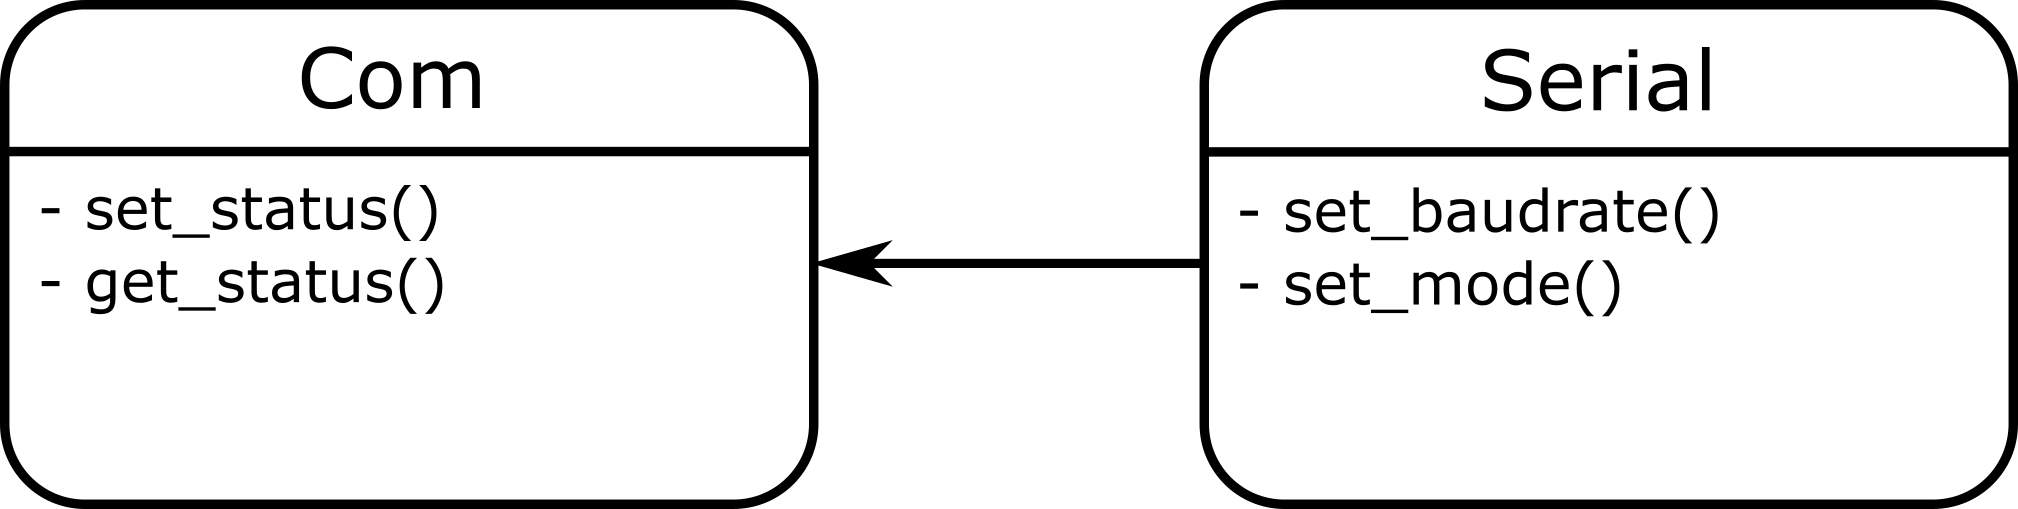
\includegraphics[scale=0.65]{../Grafiken/einfache_vererbung.png}
	\caption{Einfache Vererbung}
	\label{fig:32}
\end{figure}

Die Verwendung von einfacher Vererbung erzeugt keiner Overhead an Speicher und verändert auch das Laufzeitverhalten des Programmes nicht. Dies ist möglich da der Compiler die Funktionen statisch Binden kann da es immer eindeutig ist welche Funktion aufgerufen werden soll. Um zu analysieren ob der Compiler keine zusätzlichen Daten einbaut überprüfen wir die Größe der Serial Klasse mit \textit{sizeof}. Das Ergebnis von sizeof(Serial) liefert 16 Byte welche sich wie in Tabelle \ref{tbl:4} beschrieben zusammensetzen.

\begin{table}[!htb]
	\centering
	\begin{tabular}{| l | c | r |}
		\hline
		\textbf{Variable}   & \textbf{Bytes}    \\ \hline
		int baudrate (Serial)        & 4				    \\ \hline
		int mode (Serial)            & 4 	    		\\ \hline
		char *buffer (Serial)       & 4		            \\ \hline
		int status (Com)       & 4  			    \\ \hline
		\textbf{sizeof(Serial)} & 16 \\ \hline

		
	\end{tabular}
	
	\caption{Sizeof(Serial)}
	\label{tbl:4}
	% Verweis im Text mittels \ref{tbl:beispieltabelle}
\end{table}

Die 16 Byte setzen sich nur aus den Member Variablen zusammen welche in den Klassen \textit{Com} und \textit{Serial} definiert wurden. Somit ist bewiesen das einfache Vererbung keinen Speicher Overheat mit sich bringt und sich identisch verhält als hätte man in C mehrere Strukturen ineinander verschachtelt. Bei der einfachen Vererbung werden die Elemente der Basisklasse einfach vor die Elemente der abgeleiteten Klasse gelegt und der Aufruf einer Elementfunktion erfolgt auch ohne zusätzlichen Overhead.   \newpage


\subsubsection{Virtuelle Methoden}
Virtuelle Methoden erlauben es einer Klasse Methoden zu überschreiben welche bereits (virtuell) in der Basisklasse definiert wurden. Jedoch führt die Verwendung von virtuellen Methoden zu einigen Schwierigkeiten da der Compiler die Methoden jetzt nicht mehr statisch Binden kann sondern zur Laufzeit ein dynamisches Binden der Methoden durchgeführt werden muss. Um dieses Problem zu lösen fügt der Compiler eine Tabelle (Virtual Function Table) ein welche die Referenz auf die zu verwendete Methode beinhaltet. Diese Tabelle wird im Konstruktor des Objektes erzeugt und muss jedes mal durchsucht werden wenn eine virtuelle Funktion aufgerufen wird. Dies hat den Nachtteil das die Tabelle zusätzlichen Speicher belegt und das Laufzeitverhalten beeinflusst wird da bei jedem Aufruf einer virtuellen Funktion zusätzlichen Code ausgeführt werden muss.\newline Um dieses Problem zu verdeutlichen erweitern wir unsere Serial Klasse so dass die virtuellen Funktionen welche in der Basisklasse \textit{Com} virtuell implementiert wurden überschrieben werden. Seit C++11 kann man mit dem Schlüsselwort \textit{override} dem Compiler explizit sagen das eine Funktion überschrieben werden soll was bei schwer auffindbaren Tippfehlern hilfreich sein kann.

\begin{figure}[!htb]
	\begin{subfigure}[b]{0.5\textwidth}
		\lstset{language=C++,caption={Klassen Implementierung}}
		\lstinputlisting{../Code_Samples/Klassen/Beispiel_V5/serial.cpp}
		\label{fig:33}
	\end{subfigure}
	%
	\begin{subfigure}[b]{0.5\textwidth}
		\lstset{language=C++,caption={Klassendefinition}}
		\lstinputlisting{../Code_Samples/Klassen/Beispiel_V5/serial.h}
		\label{fig:34}
	\end{subfigure}
\end{figure}
\newpage

Wie in Abbildung 27 ersichtlich besteht nun das Problem das man zur Laufzeit eine dynamische Bindung der Funktion \textit{send\_byte} mit Hilfe der \textit{Virtual Function Table} durchführen muss. 

\begin{figure}[h]
	\centering
	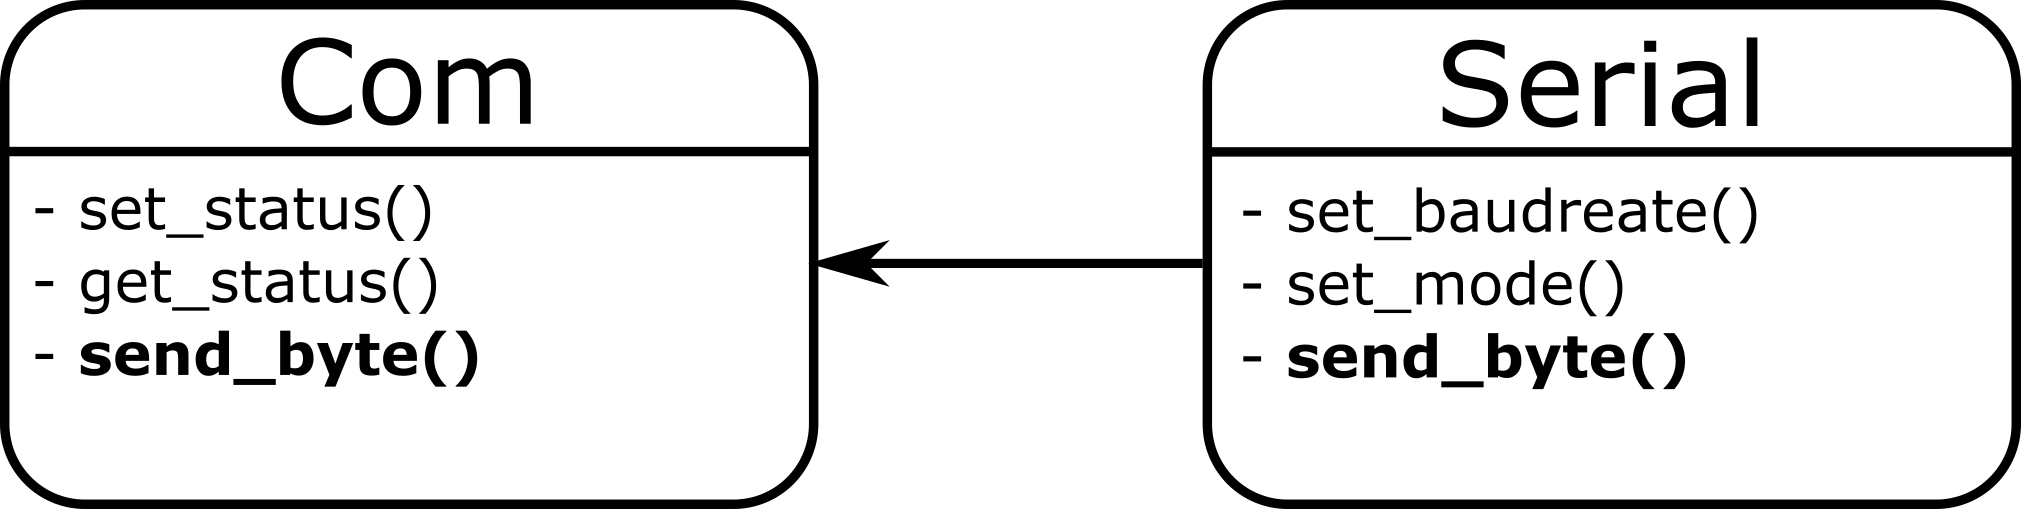
\includegraphics[scale=0.65]{../Grafiken/Virtuelle_Funktionen.png}
	\caption{Einfache Vererbung}
	\label{fig:35}
\end{figure}

Um nun zu Überprüfen wie sich virtuelle Funktionen auf den Speicherverbrauch unserer \textit{Serial} Klasse auswirken schauen wir uns das Ergebnis von \textit{sizeof(Serial)} erneut an. Nun erhält man das Ergebnis von 20 Byte welche sich wie in Tabelle 5 beschrieben zusammensetzen. Ein zusätzlicher Zeiger (4 Byte) welcher auf die \textit{Virtual Funktion Table} zeigt ist in der Basisklasse \textit{Com} dazugekommen. Die VFT Tabelle kann je nach Compiler Konfiguration in eine Sektion im ROM oder RAM gelinkt werden und beinhaltet für jede virtuelle Funktion einen Eintrag. Somit einsteht ein Speicher Overhead welcher sich durch die Größe der VFT Tabelle und dem Zeiger auf diesen zusammensetzt. 

\begin{table}[!htb]
	\centering
	\begin{tabular}{| l | c | r |}
		\hline
		\textbf{Variable}   & \textbf{Bytes}    \\ \hline
		int baudrate (Serial)        & 4				    \\ \hline
		int mode (Serial)            & 4 	    		\\ \hline
		char *buffer (Serial)       & 4		            \\ \hline
		int status (Com)       & 4  			    \\ \hline
		Pointer to VFT (Com)       & 4  			    \\ \hline
		\textbf{sizeof(Serial)} & 20 \\ \hline
		
		
	\end{tabular}
	
	\caption{Sizeof(Serial)}
	\label{tbl:5}
	% Verweis im Text mittels \ref{tbl:beispieltabelle}
\end{table}

Die Verwendung von vielen virtuellen Funktionen wirkt sich dadurch extrem negativ auf die Laufzeit des Programmes aus da bei jedem Funktionsaufruf einer virtuellen Funktion die Tabelle durchsucht werden muss und diese auch beim Anlegen eines solchen Objektes zuerst erzeugt werden muss. Der genaue Ovehead hängt natürlich von der Größe der VFT Tabelle ab.\newline \newline Ein Beispiel soll noch einmal verdeutlichen warum die VFT Tabelle benötigt wird und warum der Compiler keine statische Bindung der Funktion \textit{send\_byte} zur Übersetzungszeit durchführen kann. Im nachfolgenden Beispiel wird ein Objekt \textit{ser} vom Typ \textit{Serial} angelegt. Zusätzlich wurde eine Funktion \textit{send} implementiert die ein Zeichen auf der verwendeten Schnittelle ausgibt. Die Funktion benötigt dafür einen Parameter welcher vom Typ \textit{Com} ist um die Funktion allgemein zu halten. Somit kann die Funktion für alle Objekte verwendet werden welche von der Basisklasse \textit{Com} erben und ist unabhängig von der eigentlichen Schnittelle (I2C, SPI oder UART). Darin besteht auch jetzt das Problem da die Funktion \textit{send} ohne Hilfe der VFT nicht weiß welche \textit{send\_byte} Funktion verwendet werden soll. Dies ist auch der Grund warum sich der Zeiger welcher auf die VFT Tabelle zeigt auch immer in der Basisklasse befinden muss was wir vorher mit \textit{sizeof(Serial)} auch herausgefunden haben.

\begin{figure}[!htb]

		\lstset{language=C++,caption={Beispiel Virtuelle Funktion}}
		\lstinputlisting{../Code_Samples/Klassen/Beispiel_V5/main.cpp}
		\label{fig:36}


\end{figure}


\subsubsection{Mehrfache Vererbung}
\begin{figure}[h]
	\centering
	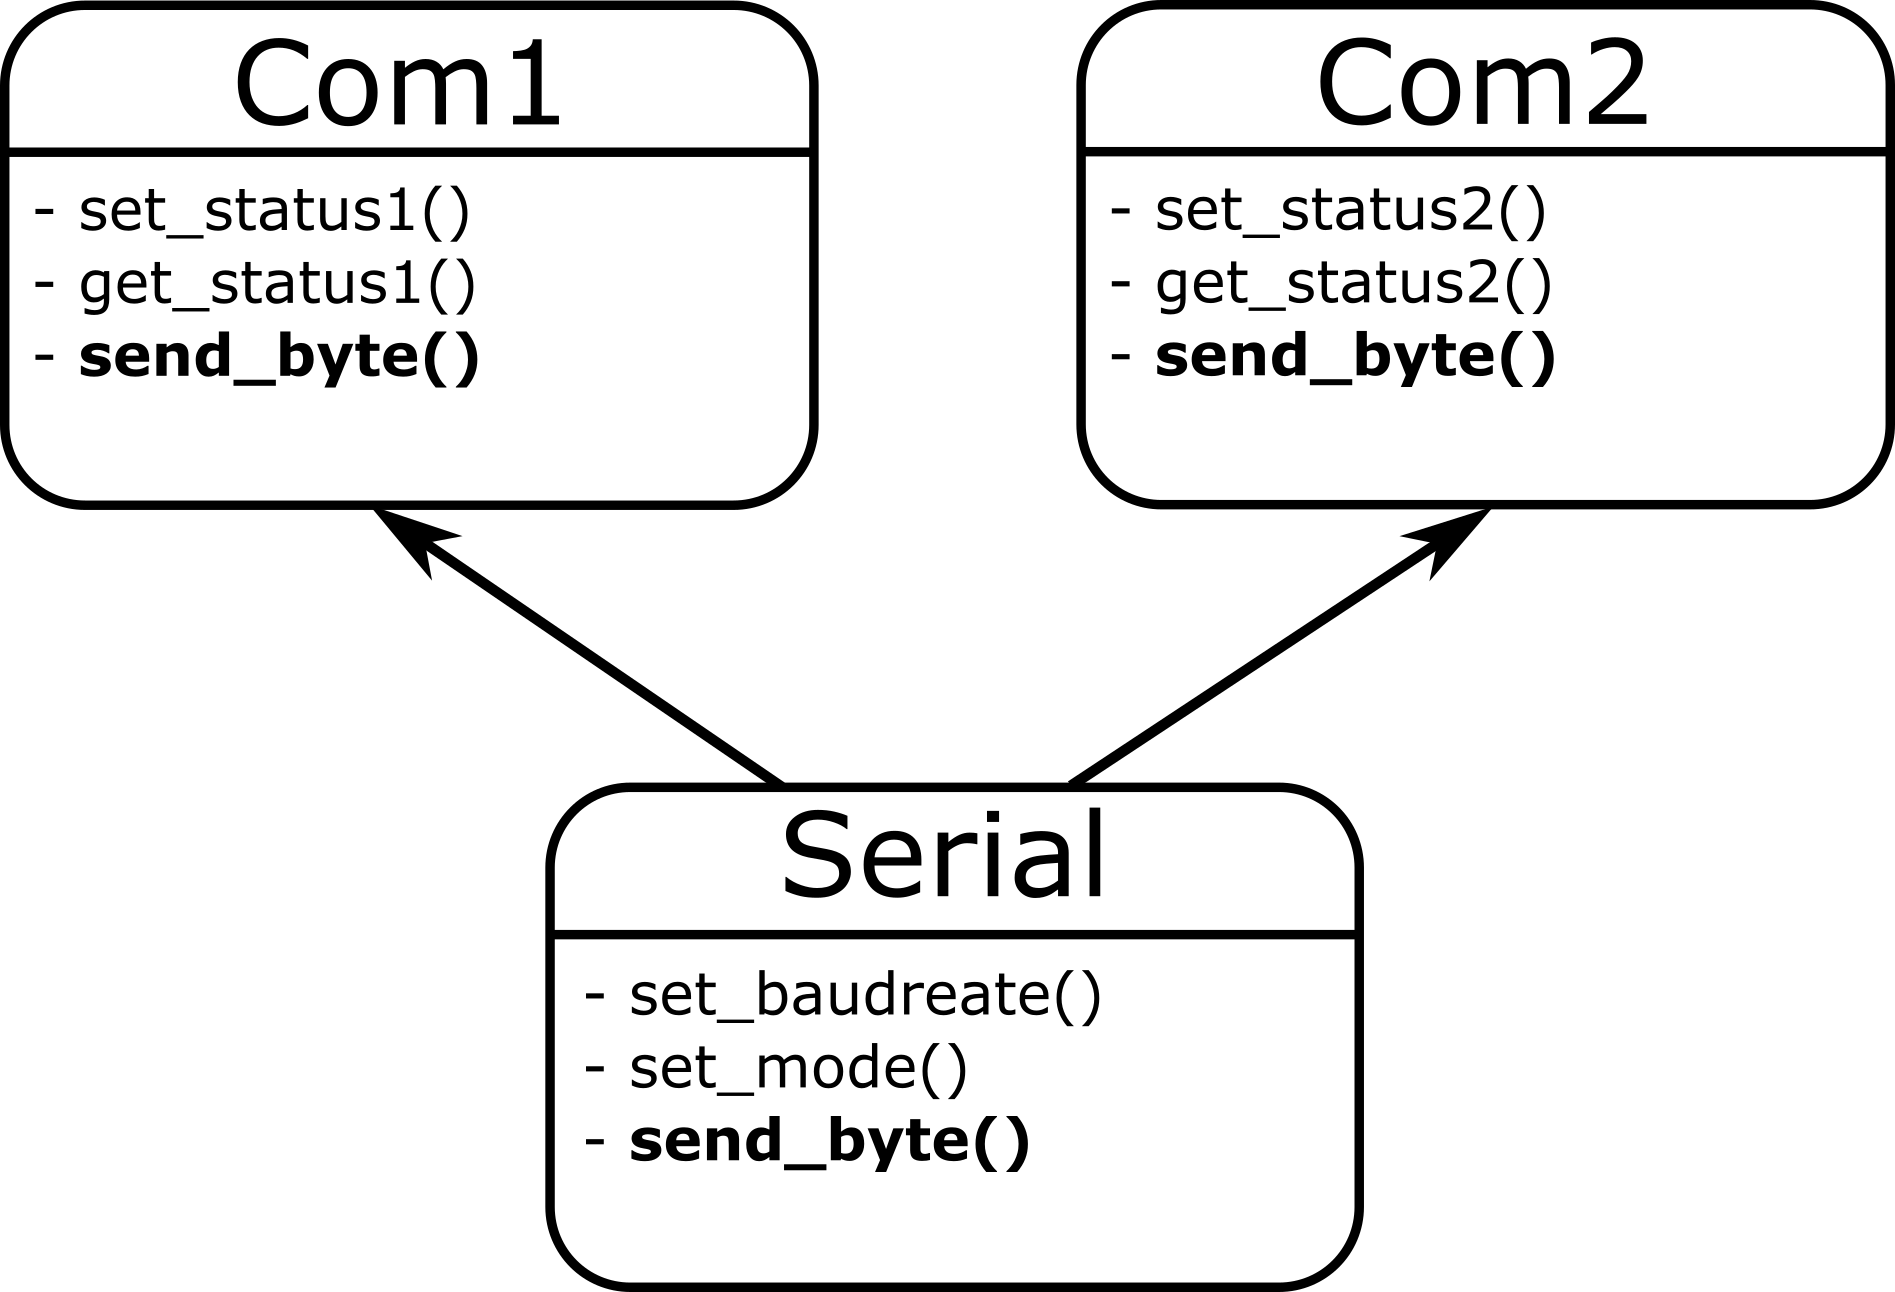
\includegraphics[scale=0.65]{../Grafiken/Mehrfache_Vererbung.png}
	\caption{Mehrfache Vererbung}
	\label{fig:37}
\end{figure}
\newpage

% Inline Methoden

% Const Methoden
\section{Operatoren Überladen}
\section{Fehlerbehandlung}
\section{Eingabe- und Ausgabestreams}



%
% Hier beginnen die Verzeichnisse.
%
\clearpage
\ifthenelse{\equal{\FHTWCitationType}{HARVARD}}{}{\bibliographystyle{gerabbrv}}
\bibliography{Literatur}
\clearpage

% Das Abbildungsverzeichnis
\listoffigures
\clearpage

% Das Tabellenverzeichnis
\listoftables
\clearpage

% Das Quellcodeverzeichnis
\listofcode
\clearpage

\phantomsection
\addcontentsline{toc}{chapter}{\listacroname}
\chapter*{\listacroname}
\begin{acronym}[XXXXX]
    \acro{STL}[STL]{Standard Template Library}
    \acro{ISO}[ISO]{International Organization for Standardization}
    \acro{ROM}[ROM]{read-only memory}
    \acro{RAM}[RAM]{random-access memory}
    \acro{RTOS}[RTOS]{Real Time Operating System}
    \acro{OS}[OS]{Operating System}
    \acro{VFT}[VTF]{irtual Funktion Table}
\end{acronym}


\end{document}